\subsubsection{SAML}\label{sec:saml}

The \acrfull{saml} is a framework for exchange of assertions containing security information between two online parties, typically an identity provider and a relying party. Similarly as XACML, \acrshort{saml} was developed by OASIS. Version 1.0 was released in 2002 and version 2.0 (latest) in 2005. The rest of this report refers to version 2.0.

The main premise of \acrshort{saml} is that the \acrfull{idp} and the protected resource/application are two separated entities. This is desired, since it enables us to manage identities centrally for multiple applications and avoids duplication of user accounts across these applications. Moreover, separating these enables both parts to specialise only in their task.

The Figure~\ref{fig:saml-architectire} illustrates the separation of these two entities. It also depicts the high-level flow of the authentication process. If the user wants to access the protected resource on the right, they first need to authenticate themselves with the \acrshort{idp}.

Another noteworthy aspect of \acrshort{saml} is the identity federation. This is achieved, when the \acrshort{idp} and the \acrshort{rp} are in different security realms, possibly operated by different organisations. As long as an agreement is established between the two, users can use their online identity, managed by the \acrshort{idp}, to access any resources outside the organisation's boundary~\cite{2008SecurityOverview}.

 \begin{figure}[ht]
    \centering
    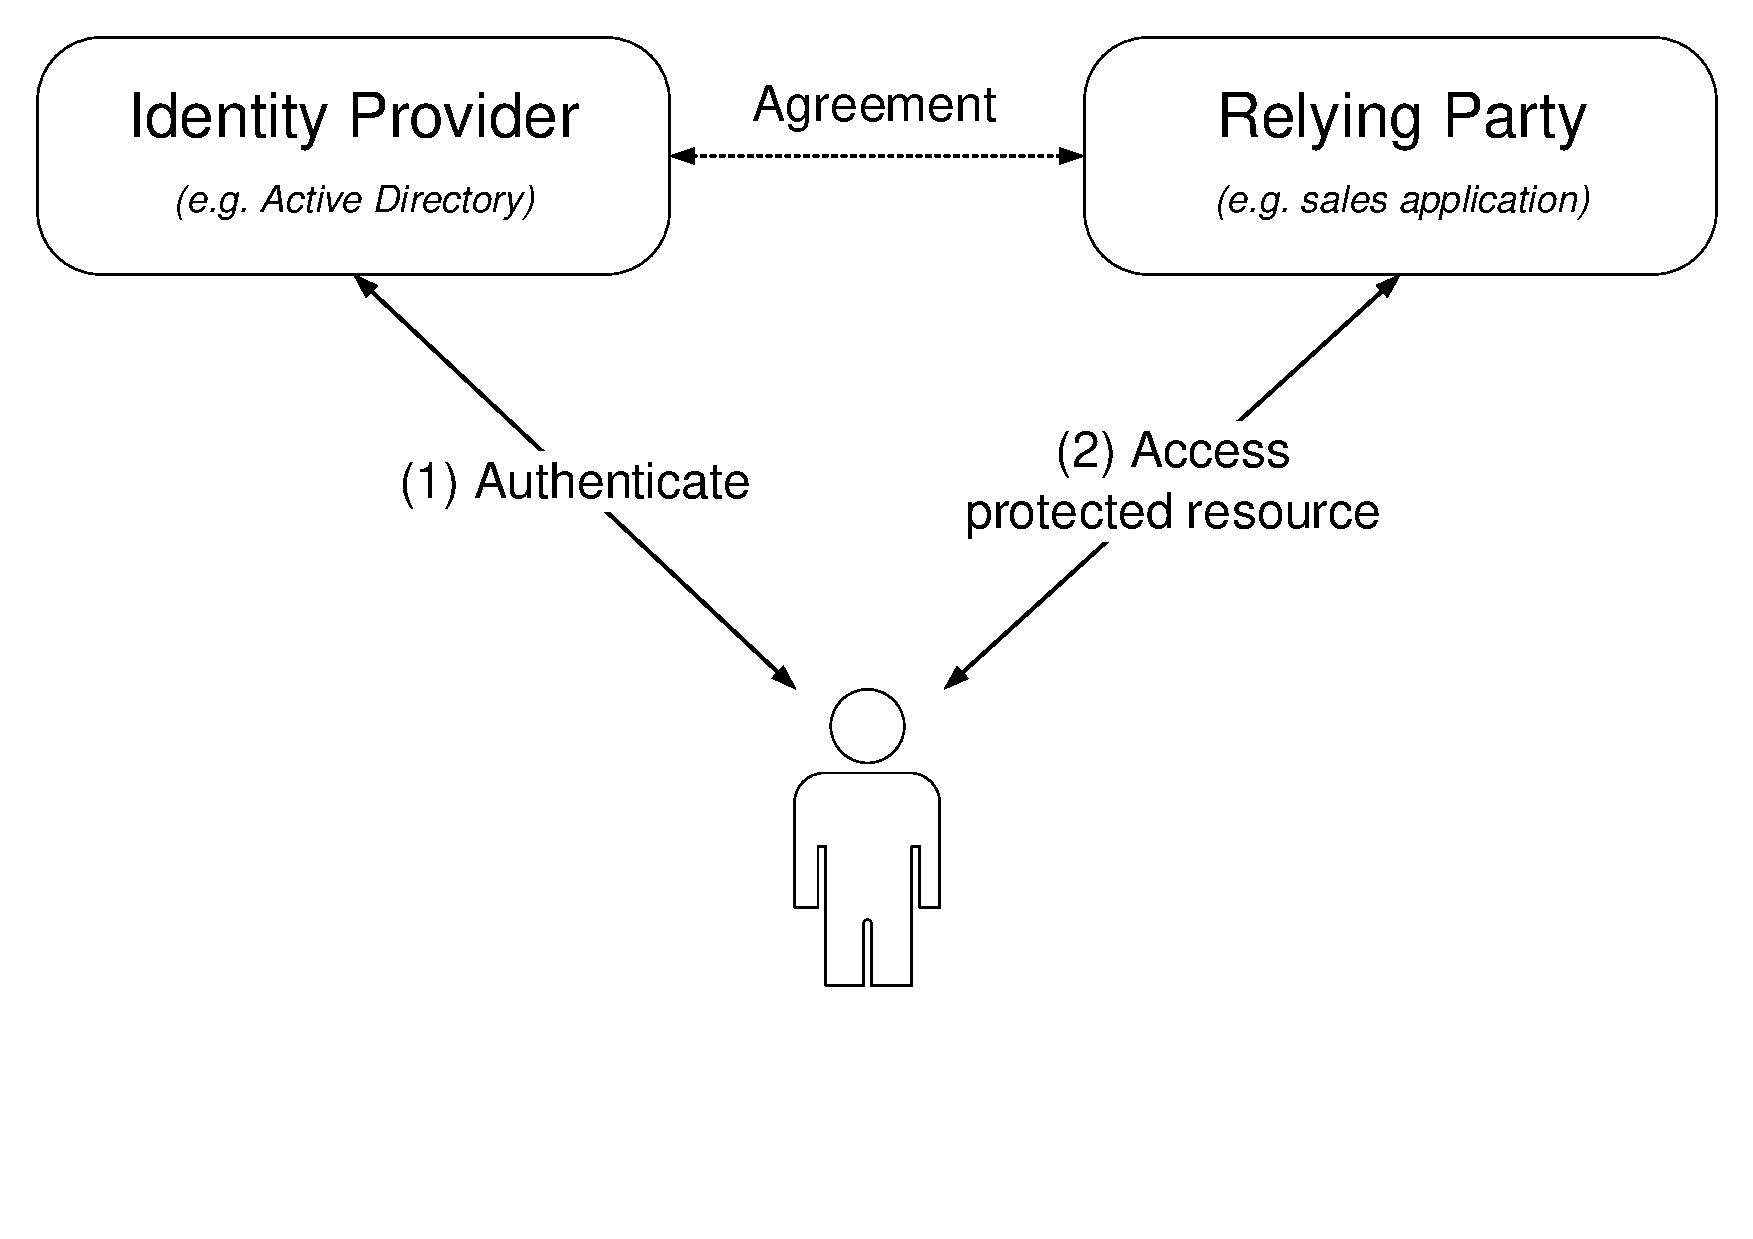
\includegraphics[width=.75\textwidth]{saml-architecture}
    \caption{The general use case of SAML, demonstrating the premise of functional separation of \acrshort{idp} and \acrshort{rp}. Taken from~\cite{2008SecurityOverview}.}
    \label{fig:saml-architectire}
\end{figure}

\paragraph{Assertions}
An assertion in \acrshort{saml} contains some security information about the \textit{subject}. Subject could be the user Bob and the associated information could be Bob's email address and job title. The security information need to be of one of following three categories:

\begin{enumerate*}[label=(\roman*)]
    \item \textit{Authentication statements} describe the means and the timestamp of the authentication carried out by the asserting party;
    \item \textit{Attribute statements} provide information about the subject; and
    \item \textit{Authorisation decision statements} describes what the subject is permitted to access in the system.
\end{enumerate*}

While \acrshort{saml} is widely adopted in the industry and is considered generally secure, numerous security flaws have been identified over time. Most of these arose from improper implementation of the protocol and have been patched since discovery~\cite{Krawczyk2014SecureAttacks}. The vulnerabilities included XML signature wrapping, assertion eavesdropping~\cite{Chen2014Environment-BoundAssertions} and XML parsing issues~\cite{Degges2018AVulnerability}.